\sub{Redux Offline}
``Persistenter Redux store für \it{reasonaboutable}\texttrademark ~Offline-First Anwendungen``. \\
Ist ein eigenständiger Statuscontainer und kann mit jeder Webanwendung angewandt werden, die sich \it{deklarativ auf Basis einer einzigen Datenquelle rendern lässt}, wie beispielsweise React\footnote{JavaScript Bibliothek: \url{https://reactjs.org/}}, Vue\footnote{JavaScript Framework: \url{https://vuejs.org/}}, oder Angular\footnote{JavaScript Framework: \url{https://www.angular.io}}~\cite{redux-offline-compabilaty}.\\
ist eine experimentelle Bibliothek die auf \it{battle-tested} patterns der Offline-First Architektur aufbaut\\
\sc{Redux Offline} verspricht nicht, die Webanwendung offlinefähig zu machen. Um \it{assets}(Bilder, Skripte etc) zwischenzuspeichern, muss zusätzlich noch ein ServiceWorker implementiert sein.\\
Benutzt redux-persist und redux-optimist.\\
Bei jeder Änderung wird der Redux store auf dem Datenträger gespeichert, und bei jedem Start automatisch neugeladen. (Standardmäßig IndexedDB, localForage, AsyncStorage)\\
Eine mit \sc{Redux Offline} erstellte Anwendung funktioniert ohne weitere Anpassung offline im Lesemodus. Also wenn die benutzende Person vom (Redux-)Status lesen möchte.
Um auch im Schreibmodus offline zu funktionieren, werden alle Netzwerkgebundenen Aktionen in einem Store-internem \gls{Queue} gespeichert. Dann erstellt \sc{Redux Offline} einen Unterbaum \tt{offline}, wo unter anderem der internen Status und ein Array namens \tt{outbox} verwaltet wird. Um diese Aktivitäten bei Internetverbindung ausführen zu können, müssen alle notwendigen Daten Plus Metadaten gespeichert werden. Die Metadaten sind für die Information zuständig, was davor oder danach passieren soll. Es gibt drei Metadaten die \sc{Redux Offline} interpretieren kann:\\
\tt{meta.offline.effect} - Die Daten die gesendet werden sollen?\\
\tt{meta.offline.commit} - Aktion die ausgeführt wird sobald Daten erfolgreich gesendet wurden\\
\tt{meta.offline.rollback} - Aktion die bei permanent fehlgeschlagener Internetverbindung
~\cite{redux-offline-gh}
\begin{figure}[H]
  \centering
  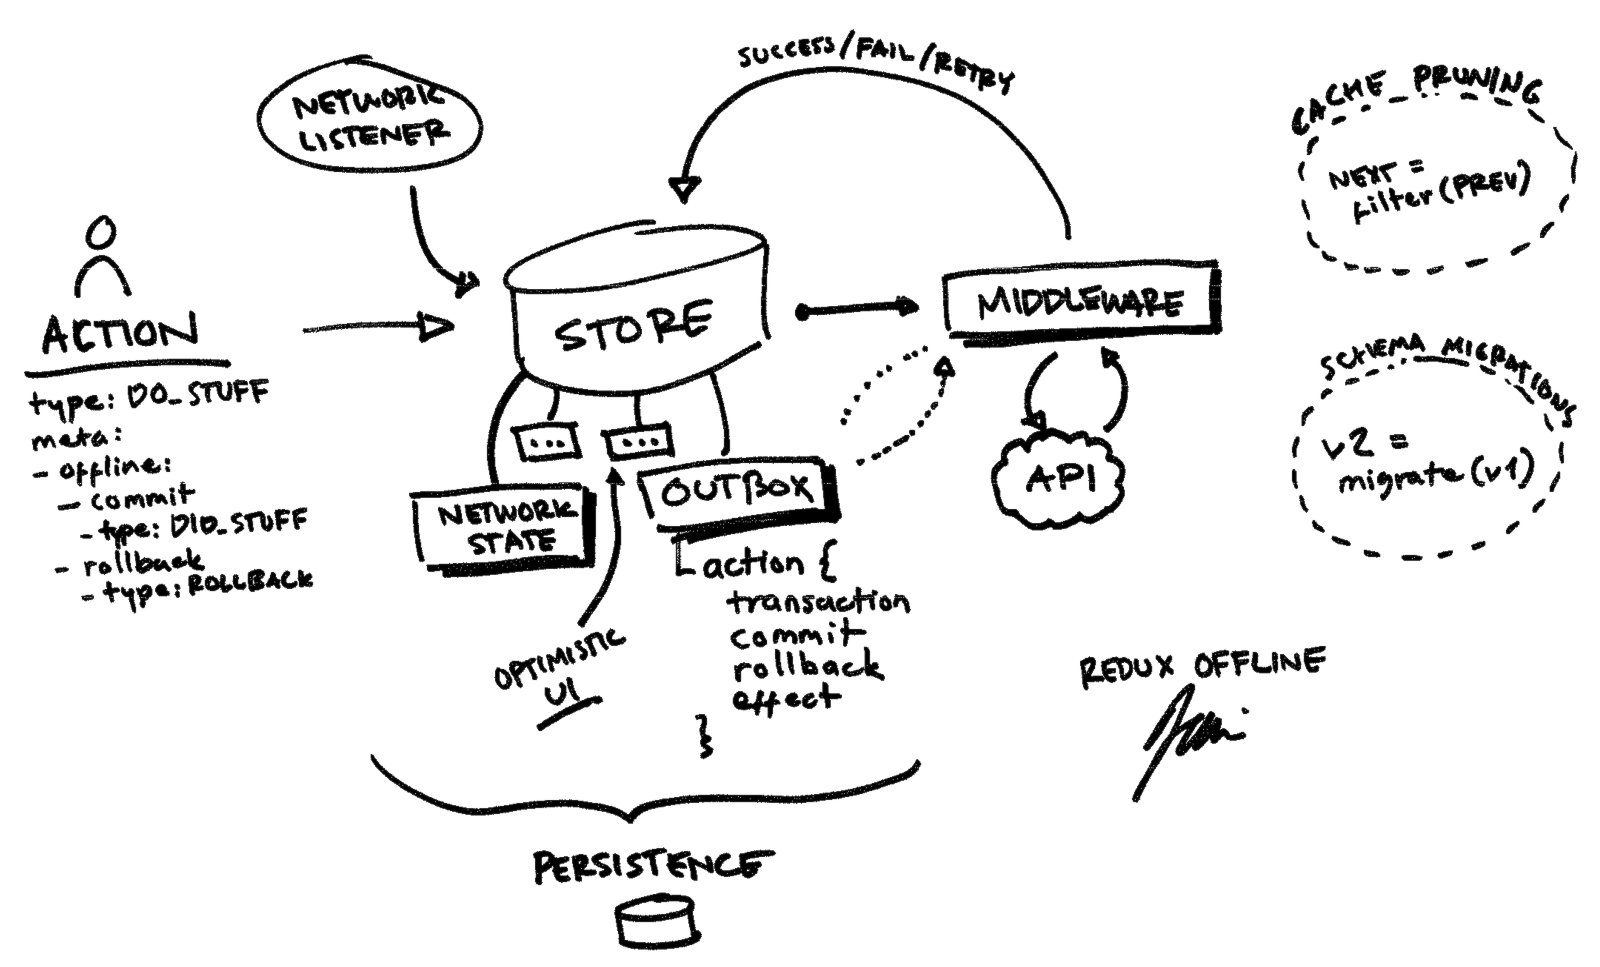
\includegraphics[width=\textwidth]{redux-offline}
  \grayRule
  \caption[Redux Offline]{Redux Offline Architektur\\\\~Quelle:~\cite{redux-offline}}
  \label{fig:redux-offline}
\end{figure}
Die grundlegende Idee hinter Redux Offline ist, dass der \sc{Redux store} die Datenbank ersetzt/ist. Jede Aktion die benötigt wird um offline zu arbeiten, wird im \sc{store} persisiert und durch die \tt{meta.offline} -Daten weiß die Anwendung was online zu tun ist. Wie die Grafik \ref{fig:redux-offline} (links) zeigt, wird jede (offline-unterstützende) Aktion mit dem \tt{offline.meta} Feld dekoriert. Darin wird beschrieben, wie der \it{Netzwerkeffekt} ausgeführt werden soll (\tt{effect}) und welche Aktion ausgelöst werden soll, wenn sie erfolgreich (\tt{commit}) ist oder fehlschlägt (\tt{rollback}). Diese Offline-Aktionen werden im \sc{store}-internen \gls{Queue} gespeichert und werden, einmal online, an den Server gesendet.\\\\
\gls{UI}\\
Es umfasst netzwerkfähige \gls{API}-Aufrufe, das Persistieren des Zustands(Status), das Stapeln von Nachrichten und die Behandlung von Fehlern, Neuversuchen, \gls{optimistic UI}-Aktualisierungen, Migrationen, Cache-Bereinigung und mehr.
Weil das kompliziert sein kann, zielt \sc{Redux Offline} darauf ab, eine vernünftige Reihe von Standardverhaltensweisen zu bieten, die verwendet werden, und nach Bedarf einzeln überschrieben werden können.\\
Grundsätzlich ist das Problem, das \sc{Redux Offline} löst, kein technisches, sondern ein Architekturproblem. Architekturen können im Code implementiert werden, aber um verstanden, angewendet und nachvollziehbar zu werden, müssen sie gut kommuniziert werden. --> Dokumentation

{\large Konflikte?}
%
% redux persist
%
\subsub{redux-persist}
localStorage. github~\cite{redux-persist-gh} medium~\cite{redux-persist}
\subsub{redux-optimist}